Having a significant enhancement of the actuator's dynamic stiffness with the help of position control techniques, as seen in the previous chapter, it is possible to evaluate if a redesigned actuator with a reduced piston area would comply with its design requirements without violating the minimum dynamic stiffness necessary for flutter suppression. 

It is important to highlight that the redesigned actuator would have smaller hydraulic consumption and would be lighter than the previous design, bringing important benefits to the overall aircraft performance. 

This chapter aims to provide the results obtained with a redesigned hydraulic actuator with its position controlled by different control techniques developed in the previous chapter.

\section{Rudder actuator new design}

The actuator new design was based on the original design developed in chapter 3. The new actuator design consists of:
\begin{enumerate}[i]
\item reducing piston seal by one size number (from $-328$ to $-327$);
\item maintaining rod size per original design;
\item maintaining EHSV per original design;
\item no change in kinematics: stroke, RLC triangle per original design.
\end{enumerate}

Tables~\ref{table:Final_Newdesign} and~\ref{table:Final_Newmargin} illustrate the new actuator design. As expected, the design has a negative margin for dynamic stiffness requirement and a smaller stall load due to the reduced actuator area. The new piston and rod seal size are displayed on table~\ref{table:Final_Newdesign}, they determine a reduction of $18.10\%$ of the actuator original area.

\begin{table}[H]
    \captionof{table}{Rudder Actuator New design}
    \label{table:Final_Newdesign}
	\centering
    \begin{tabular}{|c|c|}
    \hline
    \multicolumn{2}{|c|}{Final Actuator New Design} \\ \hline
    Piston Seal number & 327           \\ \hline
    Rod Seal number & 221 \\ \hline
    Actuator area ($A_{act}$) & $1.901 in^2$ \\ \hline
        \end{tabular}

\end{table}

\begin{table}[H]
    \captionof{table}{New Rudder Actuator against Requirements}
    \label{table:Final_Newmargin}
	\centering
    \begin{tabular}{|c|c|c|c|}
    \hline
    \multicolumn{4}{|c|}{New Actuator Design Margin} \\ \hline
    Design parameter & Requirement & New Design & Margin ($\%$) \\ \hline
    Stall load ($lbf$) & $4545.57$ & $5417.85$ & $19.20$ \\ \hline
    $K_{act}(N/m^2)$ & $1.79 E+7$  & $1.47 E+7$ & $-17.88$ \\ \hline
    \end{tabular}

\end{table}

\section{Actuator Redesign Performance}

Once the previous actuator new design is concluded, the new design validation against requirements is performed by simulation. The actuator performance for time and frequency response and the actuator's dynamic stiffness are presented in this section for different control loop configurations:
\begin{enumerate}[i]
\item Proportional controller 
\item Proportional-Derivative controller 
\item Partial-State Feedback controller 
\item Full-State Feedback controller 
\end{enumerate}

All control loops are digital implementation, except for the full-state feedback controller, which is an analog implementation.

The control gains for the modern controllers were set based on the previous development described in chapter 4 and based on an updated linear model. The digital controller gains were not modified, because the gains set in chapter 4 presented a good performance for this actuator.

\begin{table}[H]
    \captionof{table}{Classical controller gains}
    \label{table:pid_tested2}
	\centering
	\resizebox{6cm}{!} {
    \begin{tabular}{|l|c|c|}
    \hline
    \multicolumn{3}{|c|}{P and PD controller design} \\ \hline
    Parameter & P & PD \\ \hline
    $K_p$ & $ 40 $ & $40$ \\ \hline
    $K_d$ & $0.0$ & $0.7$ \\ \hline
    \end{tabular}}

\end{table}

The modern controller gain matrix are:
\begin{center}
$K_{gain_{full}}= \begin{bmatrix}
2.708\cdot10^1 & 4.855\cdot10^{-3} & 1.475\cdot10^{-6} & 2.035\cdot10^{-4} & 7.332\cdot10^1 & -4.809\cdot10^{-3}\\
\end{bmatrix}$
\end{center}
\begin{center}
$K_{gain_{partial}}= \begin{bmatrix}
2.708\cdot10^1 & 0 & 0 & 2.035\cdot10^{-4} & 7.332\cdot10^1 & 0\\
\end{bmatrix}$
\end{center}


\subsection{Time Response}

The step response of the new actuator for different control strategies can be observed in figure~\ref{fig:time_newdesign}.

\begin{figure}[H]
\centering
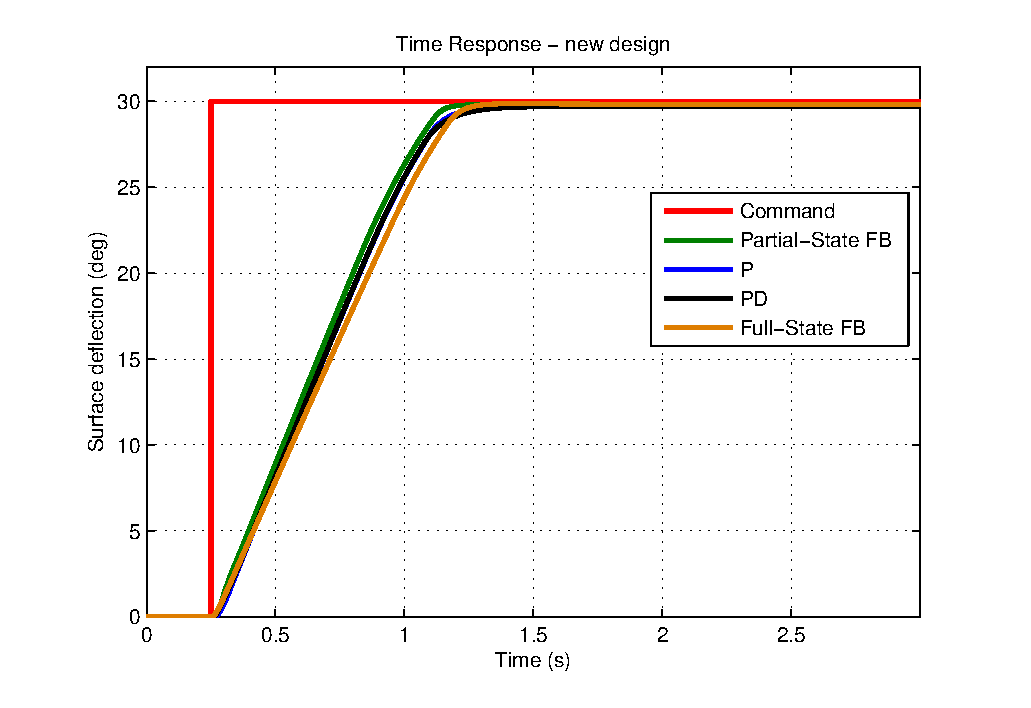
\includegraphics[scale=0.95]{figs/cap6_time}
\caption{Time Response - Different controllers - new design}
\label{fig:time_newdesign}
\end{figure}

Table~\ref{table:newdesign_time_compliance} summarize the time response performance for different controllers. All time responses are compliant with requirements. The pure proportional and the proportional-derivative controllers present the higher settling time and a similar nominal surface rate and steady state error. The modern controllers have a better settling time performance and a smaller steady state error than the classical strategies. However, the full-state feedback has the smallest average rate among all controllers. None of the control strategies determines a surface position overshoot in the step response.

\begin{table}[H]
    \captionof{table}{Rudder Actuator New Design Time Response Requirements Compliance}
    \label{table:newdesign_time_compliance}
	\centering
	\resizebox{16cm}{!} {
    \begin{tabular}{|l|c|c|c|c|c|}
    \hline
    \multicolumn{6}{|c|}{Time Response Performance} \\ \hline
    Design parameter & Requirement & P & PD & Partial & Full \\ \hline
    Settling time (ms) & $ < 850 $ & $724$ & $761$ & $640$ & $715$ \\ \hline
    Steady State error ($\%$) & $< 1$ & $0.43$ & $0.43$ & $0.32$ & $0.31$   \\ \hline
    Overshoot ($\%$) & $< 10 $  & $0.0$ & $0.0$ & $0.0$ & $0.0$  \\ \hline
    Minimum Average rate ($deg/s$) & $> 32$ & $35.23$ & $35.22$ & $35.81$ & $32.89$ \\ \hline
    Maximum Average rate ($deg/s$) & $< 36$ & $35.23$ & $35.22$ & $35.81$ & $32.89$   \\ \hline
    \end{tabular}}

\end{table}

The modern controllers present a step response performance quite similar to the classical strategies, highlighting a very good settling time and a small steady state error.

\subsection{Frequency Response}

The new actuator frequency response is illustrated in figure~\ref{fig:freq_newdesign}.

\begin{figure}[H]
\centering
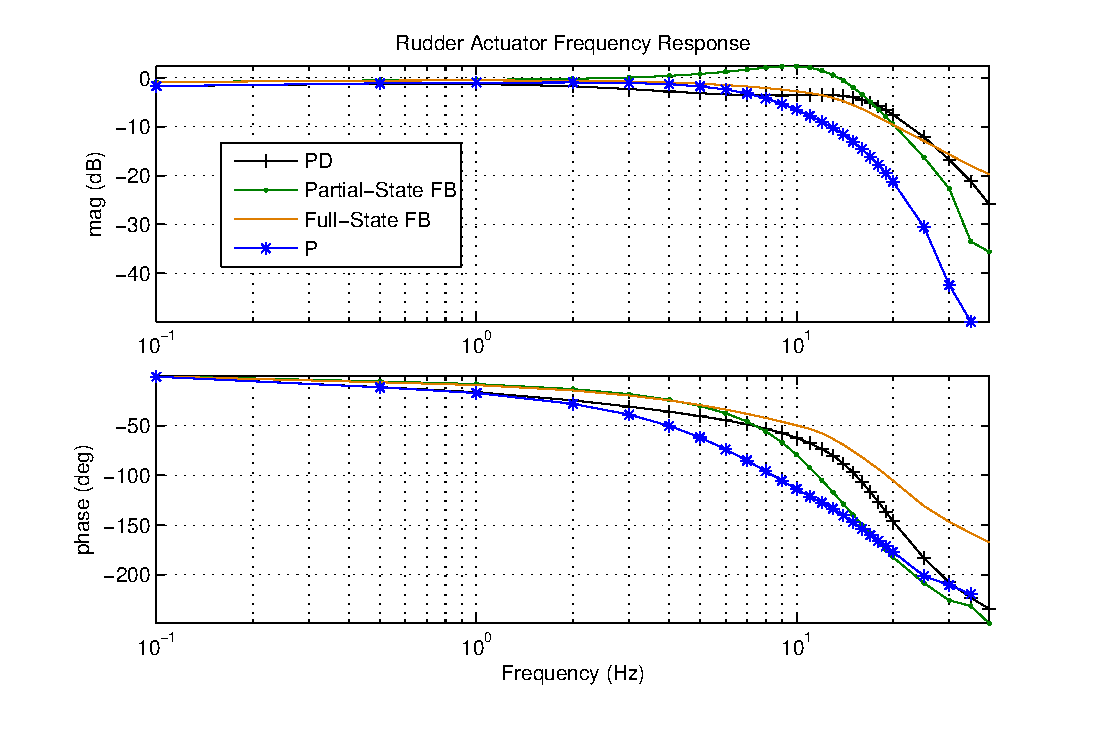
\includegraphics[scale=0.85]{figs/cap6_freq}
\caption{Frequency Response - Different controllers - new design}
\label{fig:freq_newdesign}
\end{figure}

From table~\ref{table:newdesign_freq_compliance}, it is possible to conclude the proportional gain has the best gain margin among all the implemented control strategies, but with the worst bandwidth among the control strategies evaluated. All the controllers determine a frequency response with an infinite phase margin except for the partial-state feedback strategy. In addition, the partial-state feedback and the PD controllers have a large bandwidth (around $16 Hz$) at the expense of gain margins. The full-state feedback presents a very good bandwidth (around 12 Hz) with a gain margin very close to the proportional controller.

\begin{table}[H]
    \captionof{table}{Rudder Actuator New Design - Frequency Response Requirements Compliance}
    \label{table:newdesign_freq_compliance}
	\centering
	\resizebox{14cm}{!} {
    \begin{tabular}{|c|c|c|c|c|c|}
    \hline
    \multicolumn{6}{|c|}{Frequency Response Performance} \\ \hline
    Design parameter & Requirement & P & PD & Partial & Full \\ \hline
    Gain margin (dB) & $ \geq 10 $ & $22.36$ & $11.70$ & $8.96$ & $22.07$ \\ \hline
    Phase margin ($deg$) & $ \geq 45$ & $inf$ & $inf$ & $56.80$ & $inf$ \\ \hline
    Bandwidth (Hz) & $None$ & $8.43$ & $16.36$ & $16.30$ & $12.61$ \\ \hline
    \end{tabular}
    }

\end{table}

\subsection{Dynamic Stiffness}

The new actuator's dynamic stiffness response is presented in figure~\ref{fig:ds_newdesign}.

\begin{figure}[H]
\centering
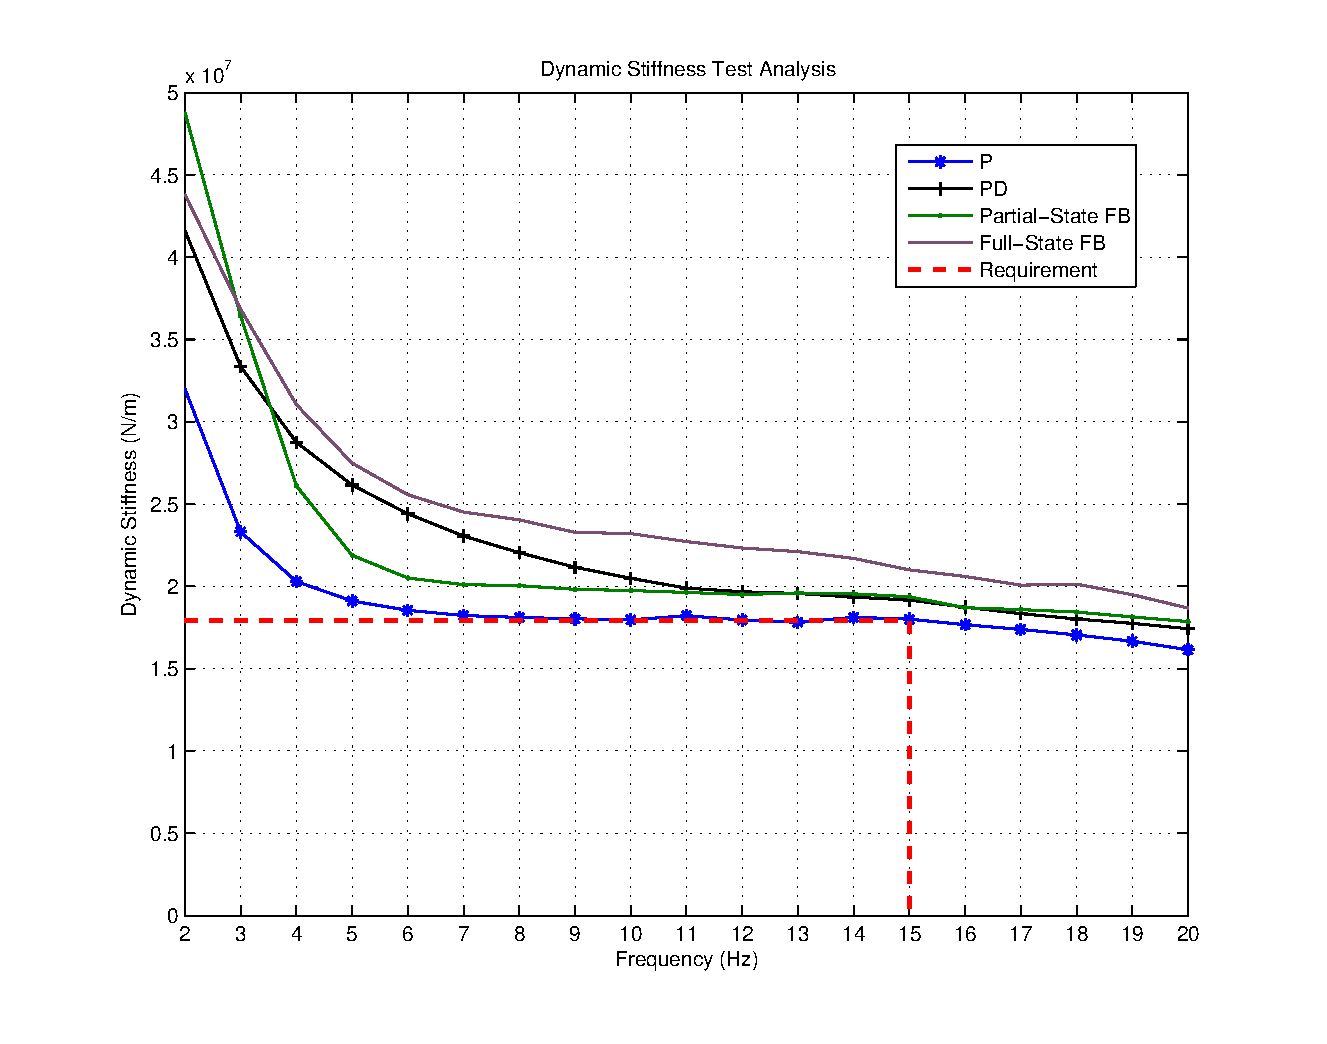
\includegraphics[scale=0.75]{figs/cap6_ds}
\caption{Dynamic Stiffness - Different controllers - new design}
\label{fig:ds_newdesign}
\end{figure}

As expected the simple proportional gain violates the requirement at infinite frequency (15 Hz). The PD and partial-state feedback present a better performance with a dynamic stiffness enhancement over the entire frequency range, as can be seen in figure~\ref{fig:ds_newdesign}. The full-state feedback presents the highest dynamic stiffness enhancement in the frequency range above 10 Hz and exceed the requirement in all the frequency range.

It can be concluded that the reduced size actuator with modern control strategies (full-state and partial-state feedback) is compliant with all time and frequency response requirements and has a dynamic stiffness response that exceeds the flutter suppression requirement.
%
%\begin{figure}[H]
%\centering
%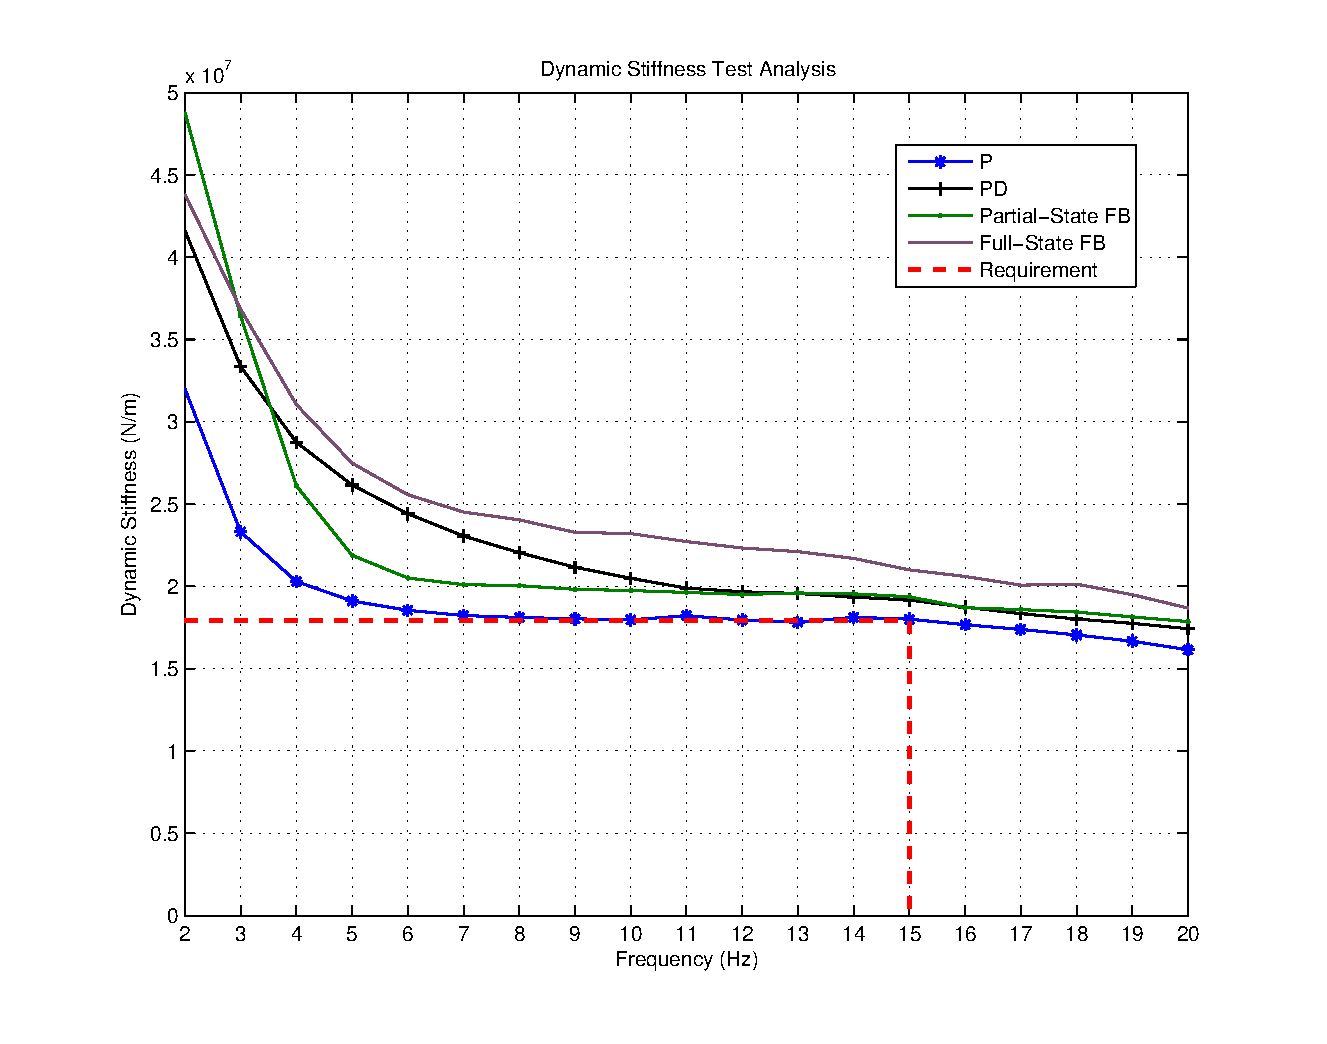
\includegraphics[scale=1.0]{figs/cap6_ds2}
%\caption{Dynamic Stiffness zoom - Different controllers - new design}
%\label{fig:ds_newdesign2}
%\end{figure}

\section{Actuator Design Comparison}

In this section, it is performed a performance comparison between the old rudder actuator, a preliminary design, with a proportional control loop (the aerospace industry standard solution) and the new actuator, an optimal design, with a reduced area and full-state feedback controller.

Table~\ref{table:design_comp} presents the comparison the main requirements and characteristics of the both actuator solutions. 

\begin{table}[H]
    \captionof{table}{Rudder Actuator New Design Frequency Response Requirements Compliance}
    \label{table:design_comp}
    \centering
	\resizebox{16cm}{!} {
    \begin{tabular}{|c|c|c|c|c|c|}
    \hline
    \multicolumn{5}{|c|}{Performance Comparison} \\ \hline
    Design parameter & Requirement & Preliminary design & Optimal design & $\Delta$ ($\%$) \\ \hline
    Settling Time (ms) & $ < 850 $ & $690$ & $715$ & $+3.62$\\ \hline
	Nominal Rate ($deg/s$) & $[32,36]$ & $34.94$ & $32.89$ & $-5.87$\\ \hline
	Steady State Error ($\%$) & $< 1$ & $0.18$ & $0.31$ & $NA$\\ \hline
	Overshoot ($\%$) & $< 10 $ & $0.0$ & $0.0$ & $0.0$\\ \hline
	Gain margin (dB) & $ \geq 10 $ & $18.38$ & $22.07$ & $+20.07$\\ \hline
    Phase margin ($deg$) & $ \geq 45$ & $inf$ & $inf$ & $NA$\\ \hline
    Bandwidth (Hz) & $None$ & $6.60$ & $12.61$ & $+91.06$\\ \hline
	Dynamic Stiffness margin $@15Hz$ ($\%$) & $NA$ & $24.2$ & $17.3$ & $NA$ \\ \hline
	Piston Area ($in^2$) & $NA$ & $2.32$ & $1.90$ & $-18.10$\\ \hline
	Seal size number & $NA$ & $328-221$ & $327-221$ & $NA$ \\ \hline
	Average Flow (gpm) & $NA$ & $3.64$ & $2.79$ & $-23.35$\\ \hline
    \end{tabular}
    }

\end{table}

The new design presents a very similar step response performance compared with the old actuator. The new nominal rate is a little lower but is still compliant with no overshoot. The new actuator's frequency response performance is better than the old one, having a bigger gain margin and bandwidth, while maintaining an infinite phase margin. The piston area is around $18\%$ smaller than the original actuator, and the hydraulic flow consumption $23\%$ smaller than the first design. In addition, the new design has a very good dynamic stiffness margin at the critical infinite flutter frequency (15 Hz) around $17\%$, which is just a little bit smaller than the original margin from the first actuator design.

\begin{figure}[H]
\centering
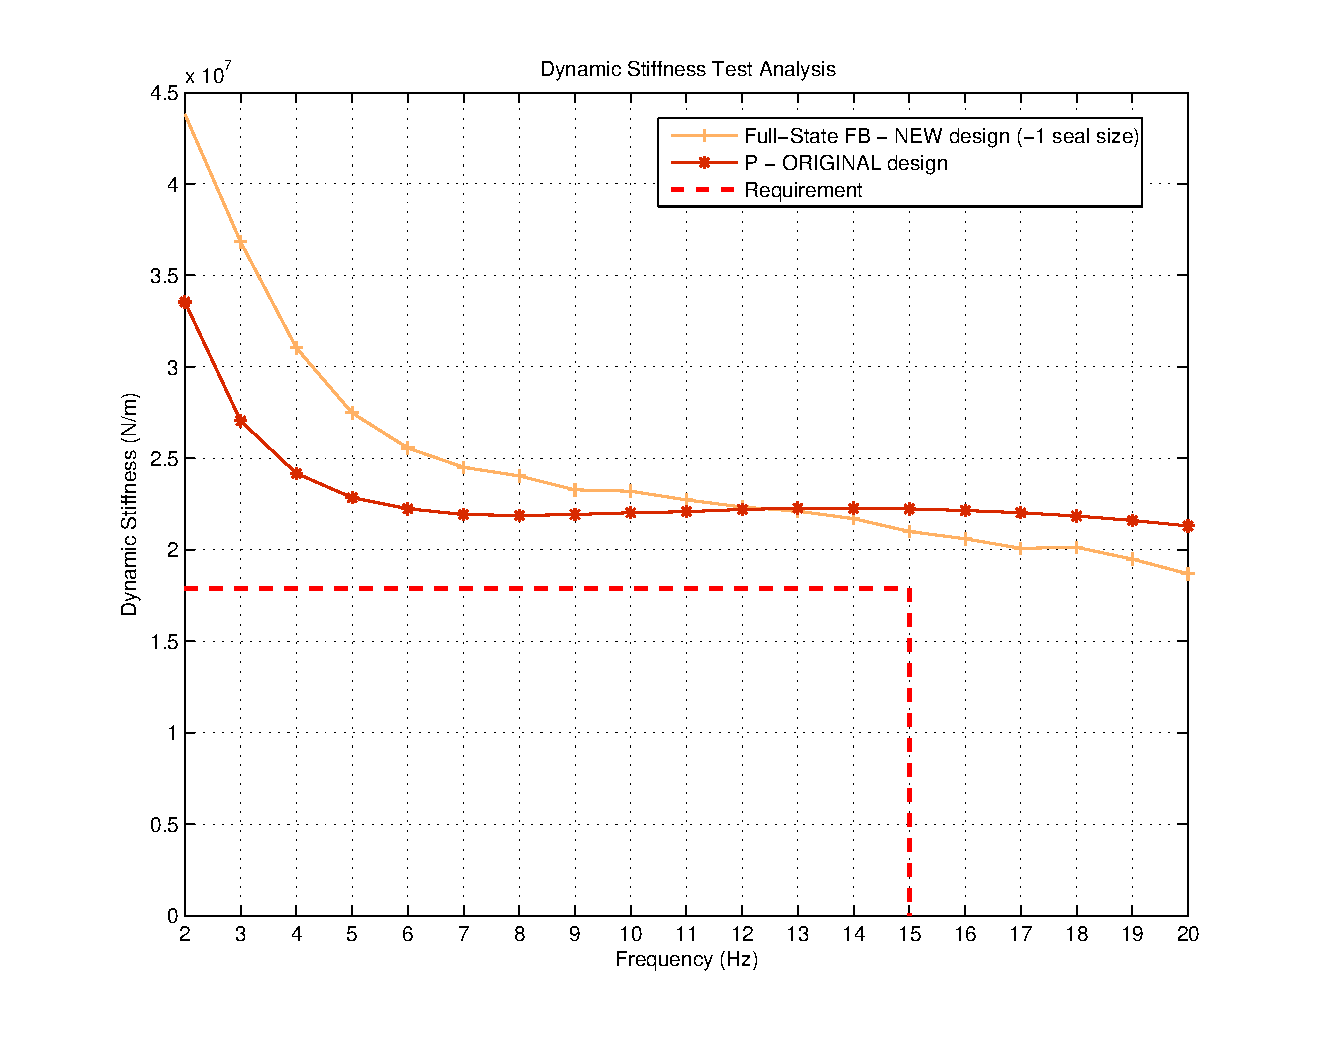
\includegraphics[scale=0.75]{figs/cap6_ds_comp}
\caption{Dynamic Stiffness - Preliminary vs. Optimal design comparison}
\label{fig:ds_newdesign2}
\end{figure}